\documentclass[a4paper, 11pt, oneside]{article}

\usepackage[utf8]{inputenc}
\usepackage[T1]{fontenc}
\usepackage[english]{babel}
\usepackage{array}
\usepackage{shortvrb}
\usepackage{listings}
\usepackage[fleqn]{amsmath}
\usepackage{amsfonts}
\usepackage{fullpage}
\usepackage{enumerate}
\usepackage{graphicx}
\usepackage{alltt}
\usepackage{indentfirst}
\usepackage{eurosym}
\usepackage{titlesec, blindtext, color}
\usepackage[table,xcdraw,dvipsnames]{xcolor}
\usepackage[unicode]{hyperref}
\usepackage{url}
\usepackage{float}
\usepackage{subcaption}
\usepackage[skip=1ex]{caption}

\definecolor{brightpink}{rgb}{1.0, 0.0, 0.5}

\usepackage{titling}
\renewcommand\maketitlehooka{\null\mbox{}\vfill}
\renewcommand\maketitlehookd{\vfill\null}

\newcommand{\ClassName}{ELEN-0060: Information and Coding Theory}
\newcommand{\ProjectName}{Project 2 - Source coding, data compression and \\ channel coding}
\newcommand{\AcademicYear}{2021 - 2022}

%%%% First page settings %%%%

\title{\ClassName\\\vspace*{0.8cm}\ProjectName\vspace{1cm}}
\author{Maxime Goffart \\180521 \and Olivier Joris\\182113}
\date{\vspace{1cm}Academic year \AcademicYear}

\begin{document}

%%% First page %%%
\begin{titlingpage}
{\let\newpage\relax\maketitle}
\end{titlingpage}

\thispagestyle{empty}
\newpage

%%%%%%%%%%%%%%%%%%%%%%%%%%%%%%%%%%%%%%%%%%

%%% Table of contents %%%
%\tableofcontents
%\newpage

%%%%%%%%%%%%%%%%%%%%%%%%%%%%%%%%%%%%%%%%%%

% CONTENT %


%%%%%%%%%%%%%%%%%%%%%%%%%%%%%%%%%%%%%%%%%%
\section{Source coding and reversible data compression}

\subsection{Question 5}
\paragraph{}First, we can compute the marginal probability distribution of all the symbols based on the given Morse text. The distribution is:
\begin{table}[H]
    \centering
    \begin{tabular}{|c|c|c|c|c|}
    \hline
    \textbf{Symbol}      & . & - & \_ & / \\ \hline
    \textbf{Probability} & 0.43378 & 0.28706 & 0.21452 & 0.06464 \\ \hline
    \end{tabular}
    \caption{Marginal probability distribution of all the symbols}
\end{table}
Based on the distribution of probabilities, we can compute the binary Huffman code. We get the following code:
\begin{table}[H]
    \centering
    \begin{tabular}{|c|c|c|c|c|}
    \hline
    \textbf{Symbol}      & . & - & \_ & / \\ \hline
    \textbf{Huffman code} & 0 & 11 & 101 & 100 \\ \hline
    \end{tabular}
    \caption{Binary Huffman code}
\end{table}
By applying the obtained Huffman code to the Morse text, we get the encoded Morse text whose size is 2213141 bits. The original Morse text has a size of 4797160 bits. Thus, we have a compression rate of 2.16758.

\subsection{Question 6}
\paragraph{}We can compute the expected average length of the Huffman code by computing the sum for the 4 symbols of the probability of each symbol times the length of the code associated with the symbol.
We get that the expected average length is equal to 1.84538.\\
By comparing to the empirical average length of the Huffman code, we get:
$$\text{Length of encoded } / \text{ length of initial text} = 1.84538$$
This value is the same as the one for the expected average length which is logical since the expected average length was computed based on the probabilities of occurrence of each symbol based on the given Morse text.\\
By comparing to the theoretical bounds, we get that:\\
\begin{equation}
    \frac{H(S)}{log_2(q)} \leq \overline{n} \leq \frac{H(S)}{log_2(q)} + 1$ because $1.77138 \leq 1.84538 \leq 2.77138
\end{equation}
Thus, our code is optimal, because the inequation is satisfied, which was expected because Huffman codes are optimal. But, the obtained code is not absolutely optimal because $\frac{H(S)}{log_2(q)} \neq \overline{n}$.

\subsection{Question 7}
\paragraph{}For the evolution of the empirical average length of the Huffman code with respect to the lengths of the input texts, we get the following plot:
\begin{figure}[H]
    \centering
    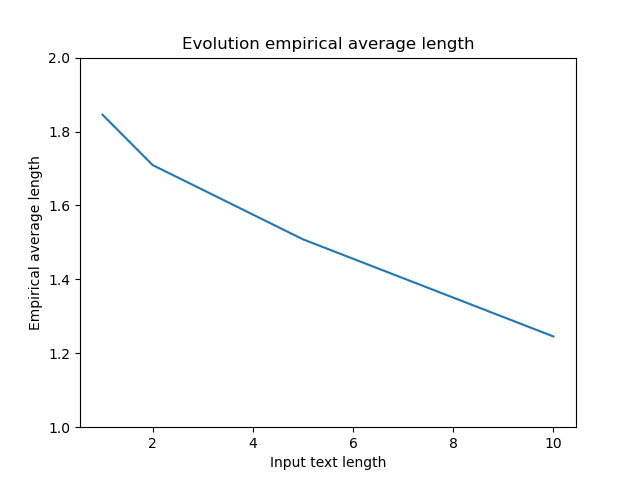
\includegraphics[scale=0.5]{q7.png}
    \caption{Evolution of empirical average length}
\end{figure}
As we can observe on the plot, the empirical average length decreases as the length of the input text increases.

%%%%%%%%%%%%%%%%%%%%%%%%%%%%%%%%%%%%%%%%%%

\end{document}